\subsection{Background \& Terminology}\label{subsec:background-&-terminology}
\subsubsection{C2KA Agents}\label{subsubsec:c2ka-agents}
Communicating Concurrent Kleene Algebra (C2KA) is a formal language intended to support the analysis of concurrent systems with communicating agents. % TODO: Ref here
\textbf{Agents} are any systems whose \textbf{behaviour} consists of discrete actions ~\cite{c2ka_foundations}.
\textbf{Stimuli} are messages passed between agents to communicate and cause changes in their behaviours.
We won't delve much further into the formal definition of C2KA and its goals,
as there are better resources for that~\cite{c2ka_foundations, implicit_interactions}.

Instead, we will identify relevant terms from a C2KA analysis that was performed on a real system~\cite{manu_cell}.
Our system of interest is a Manufacturing Cell, shown by the collaboration diagram in figure~\ref{fig:manucell-collab}.
\begin{figure}
    \centering
    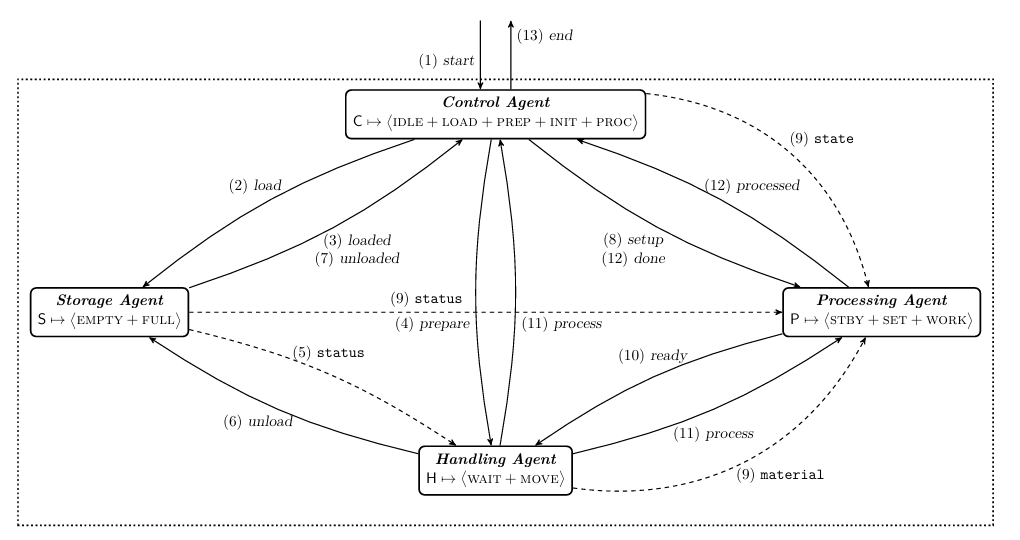
\includegraphics[scale=0.35]{manucellCollab}
    \caption{The collaboration diagram representing the Manufacturing Cell~\cite{manu_cell}}
    \label{fig:manucell-collab}
\end{figure}

In the boxes, we see the possible discrete agent behaviours, denoted by the ``+'' choice operator.
This is also how we define the \textbf{Abstract Behaviour Specification}, as seen in figure~\ref{fig:abstractmc}.
\begin{figure}
    \centering
    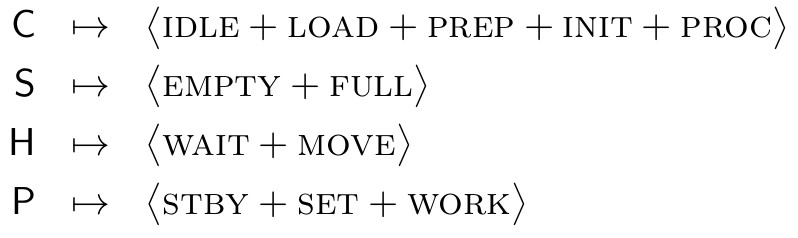
\includegraphics[scale=0.6]{abs_manucell}
    \caption{The abstract behavior specification for the system~\cite{manu_cell}}
    \label{fig:abstractmc}
\end{figure}

The solid communication arrows represent stimuli.
The stimuli are relevant for the Stimulus-Response Specification.
We break it down into its components and refer to them in this report as \textbf{Next Behaviour Mapping} (figure~\ref{fig:manucell_behav})
and \textbf{Next Stimulus Mapping} (figure~\ref{fig:manucell_stim}).
As the names may imply, these are functions which map an initial behaviour, and an input stimuli to the Agent's next behaviour, or next stimulus (respectively).
These have to be complete functions, but some papers may leave \textit{neutral mappings} empty.
These are mappings where a \textit{neutral stimulus} with no impact on agents is sent out, or the behavior remains the same.

\begin{figure}
    \centering
    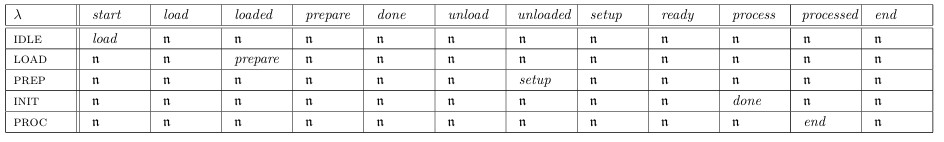
\includegraphics[scale=0.6]{manucell_stim}
    \caption{The next stimulus mapping for agent C~\cite{manu_cell}}
    \label{fig:manucell_stim}
\end{figure}
\begin{figure}
    \centering
    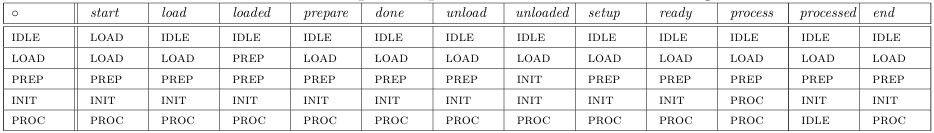
\includegraphics[scale=0.6]{manucell_behav}
    \caption{The next behavior mapping for agent C~\cite{manu_cell}}
    \label{fig:manucell_behav}
\end{figure}

The dashed arrows represent shared environmental variable information being passed.
The way these values get checked and set is defined in the \textbf{Concrete Behaviour Specification}.
These are concrete programs associated with specific behaviour, defined in Dijkstra's Guarded Command Language (GCL).
An example of this specification can be seen in figure~\ref{fig:manu_concrete} for agent C of the Manufacturing Cell.
\begin{figure}
    \centering
    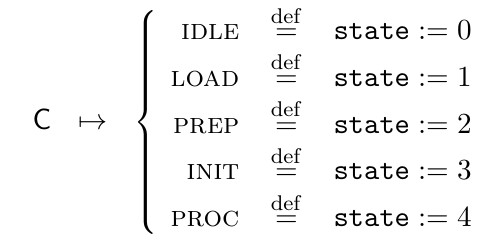
\includegraphics[scale=0.6]{manucell_concretejpg}
    \caption{The Concrete Behavior Specification for agent C~\cite{manu_cell}}
    \label{fig:manu_concrete}
\end{figure}

\subsubsection{Agents as State Diagrams}\label{subsubsec:diagram-agents}
UML State Diagrams are an informal way to represent finite state machines.
These are abstract machines that can only be in one \textbf{state} among a finite set of possible states.
To change between states, the machine establishes possible transitions triggered by \textbf{inputs}.

When we interchange state with behaviour and inputs with stimuli, we observe many similarities with C2KA\@.
A set of states of a state diagram corresponds quite well with the Abstract Behaviour Specification.
Transitions between states indicate which behaviours a stimulus can induce on a behaviour.
Paired with the ability to show outputs on a transition, we can also show the next stimulus directly on the transition.

There is even a concept for concrete programs in UML State Diagrams.
\textbf{Do Activities} refer to a concrete action that is executed while in the state.
This means we can encode the GCL in the do activity of a state to describe its Concrete Behaviour.

\subsubsection{XMI Model Exports}
To start processing a graphical model, we need a way for the computer to read it deterministically.
This is where the XML Metadata Interchange (XMI) format helps.
It is a standard used to exchange metadata information through XML, mainly for UML models.

The first goal was to be able to model in one tool and be able to pass it around to different tools.
Unfortunately, in practice, the imports do not always work cleanly.
Even our chosen modelling tool encodes additional information outside the ``.uml'' files to be able to import the diagram back in Papyrus.

The second and more relevant goal for us is its use in model-driven engineering.
This is the idea that the models should be machine-readable to be able to generate code from them.
Although this is not our purpose, we still need this property to perform our analysis and generate specifications instead.

\subsection{System Development}
\label{subsec:system-development}
% Change to User requirements?
\subsubsection{User Requirements}\label{subsubsec:user-reqs}

These User Requirements represent our original set of requirements, with minimal implementation details, and domain knowledge.
They are elicited from initial discussions with our supervisor,
and interpretations of the problem statement.
We did not establish a procedure for explicit lower level requirements after this stage.

Some limitations of this process is a lack of explicit detail, priorities, or levels of satisfaction for non-functional requirements.
Instead, we will use later stages of the system development to trace design decisions taken for these requirements.
We will also touch on priorities and possible improvements when we explain
which requirements were skipped for our current release in section~\ref{subsubsec:unsat-reqs}.

The table of requirements contains a list of User Requirements for our system,
with green states indicating satisfactory completion, and gray indicating unsatisfactory:
% Requirement table
\begin{longtable}{|l|p{2.6cm}|l|p{4.5cm}|c|}
    % First header, with label
    \caption{Set of User Requirements for U2C}\label{tab:user-reqs}\\ \hline
    \textbf{ID} & \textbf{Requirement} & \textbf{Type}  & \textbf{Description} & \textbf{State} \\ \hline
    \endfirsthead
    % Other headers, without label
    \caption{Set of User Requirements for U2C} \\ \hline
    \textbf{ID} & \textbf{Requirement} & \textbf{Type}  & \textbf{Description} & \textbf{State} \\
    \hline
    \endhead
    \hline
    % Requirements here
    1 & Input & Functional & U2C shall accept visual system models as input. & \cellcolor{green!30}  \\
    \hline
    2 & C2KA Specifications & Functional & U2C shall interpret given inputs to derive a complete C2KA agent specification. & \cellcolor{green!30}  \\
    \hline
    3 & IIAT Parameters & Functional & U2C shall interpret given inputs to derive the other required IIAT inputs. & \cellcolor{gray!30}  \\
    \hline
    4 & Output & Functional & U2C shall output its computed inputs as text files. & \cellcolor{green!30}  \\
    \hline
    5 & Minimal User Actions & Usability & U2C shall require no additional inputs from the user apart from those required to provide system models. & \cellcolor{green!30}  \\
    \hline
    6 & Modelling Tool Support & Compatibility & U2C shall support models produced by at least one chosen modelling tool (Papyrus, LucidChart, StarUML). & \cellcolor{green!30}  \\
    \hline
    7 & Modelling Language Support & Compatibility & U2C shall support visual models drawn in at least one type of modelling language (ex: UML, SysML, BPMN). & \cellcolor{green!30}  \\
    \hline
    8 & Diagram Type Support & Compatibility & U2C shall support diagrams corresponding to at least one chosen type (ex: state, collaboration, etc.). & \cellcolor{green!30}  \\
    \hline
    9 & Cross Tool Integration & Compatibility & U2C should provide options to integrate directly into tools it depends on (input producer, and output consumers). & \cellcolor{gray!30}  \\
    \hline
    10 & OS Support & Portability & U2C shall run on at least one chosen OS distribution. & \cellcolor{green!30}  \\
    \hline
    11 & Simple System Analysis Speed & Performance & U2C shall produce outputs for a simple system within one minute of execution on a chosen platform specification.
    A simple system is defined as having up to five agents, twenty stimuli, and five behaviours per agent. & \cellcolor{gray!30}  \\
    \hline
    12 & Worst Case Mitigation & Scalability & U2C should scale at a smaller rate than O($n^3$). The expected scaling factors are agents, stimuli, and agent behaviours. & \cellcolor{gray!30}  \\
    \hline
    13 & User Documentation & Maintainability & The U2C code repository shall contain a user manual detailing expected user interactions, and input formats. & \cellcolor{gray!30}  \\
    \hline
    14 & Maintainer Documentation & Maintainability & The U2C code repository shall contain documentation detailing implementation details for maintainers. & \cellcolor{green!30}  \\
    \hline
    15 & Verification Testing & Maintainability & The U2C code repository shall contain automated regression tests providing adequate coverage of the program source code. & \cellcolor{green!30}  \\
    \hline
    16 & Accurate Outputs & Accuracy & U2C shall provide deterministic outputs representing accurately what the inputs contain. & \cellcolor{green!30}  \\
    \hline
    17 & No False Positives & Reliability & U2C shall not provide outputs if it cannot find a deterministic interpretation of the given inputs. & \cellcolor{gray!30}  \\
    \hline
\end{longtable}

\subsubsection{Chosen Input Type}
The first decision to take concerning inputs was the specific diagram type to support.
This decision impacts the language, since the diagram type may be specific to one or a small set of languages.
It also impacts the modelling tool because it needs to support creating that diagram type.
Most importantly, if the diagram does not have the information we require, there is no purpose in processing it.

Recall that the information we require is related to creating C2KA agent specifications.
Our initial diagram choice was \textit{collaboration diagrams}, due to their simplicity.
When we learned more about C2KA, we realized they do not model agent behaviour very well.
Collaboration diagrams are more suited to describe a specific scenario on an entire system.
Instead, we found that having one \textbf{UML State Diagram} per agent is enough to simply capture agent specifications.
More details on this later when we break down relevant components of state diagrams in section~\ref{subsubsec:input-specification}.

By choosing UML State Diagrams, we also choose \textbf{UML} as our modelling language.
SysML could have been a close viable alternative, but we decided to choose a language we were more familiar with.
This makes it easier to implement properly for us,
but it is also related to our problem statement aiming to use modelling languages already familiar to system designers to reduce the learning curve.
Admittedly outside of software system design SysML is more prevalent, and it is feasible to support both, but we had to limit our scope.

For our modelling tool, we chose \textbf{Papyrus}.
We established evaluation criteria to evaluate different tools, and compared the most popular ones we found.
The most important requirement was machine readability.
We needed to be able to export some representation of the diagram our system could read outside the modelling tool.
Additionally, it was an advantage if it was free, popular, and had ongoing support.
We did not want the modelling tool we depended on to become a hurdle to adopt our program,
ideally we chose a tool which was already in use.
Other tools we looked at were Lucidchart, draw.io, Creately, Gliffy, UMLLet, PlantUML (all had poor export functions),
Modelio (felt hard to use), Astah UML (unpopular),
StarUML and Visual Paradigm (seemed like good alternatives, but we figured out how to use Papyrus first).

To export diagrams from Papyrus, there is an option to export \textbf{XMI files}.
They technically have a .uml file extension in papyrus, but they function the same as XMI files from other tools.
Once a diagram for an agent is finished in papyrus, we can add its XMI file to our program's \textbf{input folder}.
Once all agents are done, we can execute the program.
The user does not need to provide additional inputs.
A full workflow using our program is described in section~\ref{subsec:usage}.

The table below is a traceability summary mapping our original user requirements to the concepts refining them.
Refinements can be correlated by the bolded terms above.

\begin{table}[htbp]
\centering
\caption{Input Decision Requirement Traceability}\label{tab:input-table}
\begin{tabularx}{\textwidth}{| l | l | X |}
    \hline
    \textbf{ID} & \textbf{User Requirement} & \textbf{Refinement} \\
    \hline
    1 & Input & Visual Diagrams are given to the system through XMI file exports from supported modelling tool(s). \\ \hline
    5 & Minimal User Actions & The user puts files in an input folder, then executes the program.  \\ \hline
    6 & Modelling Tool Support & The chosen modelling tool is Papyrus. \\ \hline
    7 & Modelling Language Support & The chosen modelling language is UML. \\ \hline
    8 & Diagram Type Support & The chosen input diagram type is UML State Diagrams. \\ \hline
\end{tabularx}
\end{table}

\newpage
\subsubsection{Input Specifications}\label{subsubsec:input-specification}
Although we accept UML State diagrams, there are specific elements that our interpreter cares about.
The primary goal was to make use of essential model elements only, specifically states and transitions,
to avoid extra modelling requirements.
Unfortunately, modelling expressiveness was a smaller priority, as such
other elements may cause unexpected behaviour.
Ideally, they are ignored.
The next best case is a descriptive error gets raised and crashes the program preventing a faulty output.
In the worst case, an inaccurate specification may be generated without warning.

For the safest behaviour, we have defined a known set of valid model elements, along with usage guidelines.
At a high level, it can be summarized with the class diagram in figure~\ref{fig:supportedElems}.
\begin{figure}[ht]
          \centering
          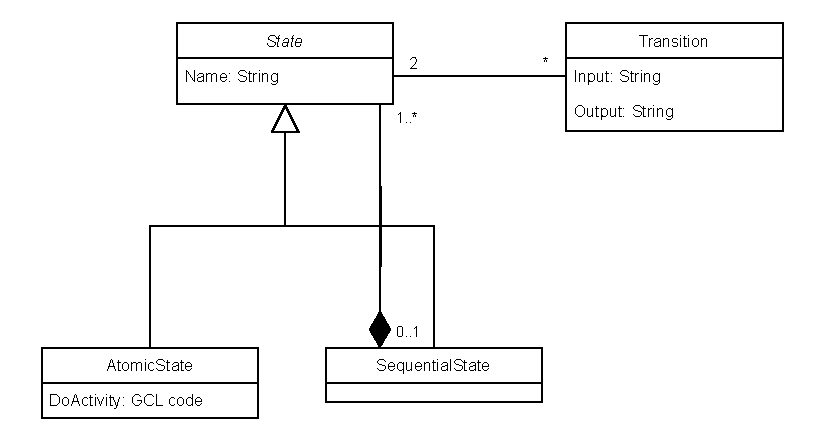
\includegraphics[width=0.5\textwidth]{supportedStateElems.drawio}
          \caption{The class diagram representation of supported diagram elements}
          \label{fig:supportedElems}
\end{figure}
\\
The first element in our state diagram is a \textbf{state}.
States describe a discrete behaviour where an invariant condition holds.
They map directly to \textit{Abstract behaviours} in C2KA\@.
\textbf{Atomic States} are states which do not contain other states.
We can see an example atomic behaviour in figure~\ref{fig:atomicbehaviour}.

\begin{figure}[ht]
    \centering
    \includegraphics[width=0.5\textwidth]{Atomicbehavior}
    \caption{A generic atomic behaviour representation}
    \label{fig:atomicbehaviour}
\end{figure}

Atomic States always have a \textbf{doActivity} property,
as they are needed for C2KA \textit{Concrete behaviours}.
doActivities need to follow Dijkstra's Guarded Command Language (GCL) notation~\cite{gcl}.
They are used to assign environmental shared variable values,
with the option to use conditional flows based on the current environment state.
Due to typesetting constraints, we had to convert the GCL operands listed in table~\ref{tab:gcl-equivalence}.
\begin{table}[htbp]
      \centering
      \caption{GCL Conversions for Modelling Tools}\label{tab:gcl-equivalence}
      \begin{tabular}{| l | l |}
          % Header
          \hline
          \textbf{Original GCL} & \textbf{Modelling Tool} \\
          % Header end
          \hline
          $\land$ & \&\& \\ \hline
          $\square$ & $|$ \\ \hline
          $\lor$ & $||$ \\ \hline
          $\rightarrow$ & $->$ \\ \hline
      \end{tabular}
\end{table}
\\

\textbf{Transitions} are links between states which describe how changes in state occur.
We use these transitions and their associated behaviours to compute \textit{Next behaviour} and \textit{Next Stimulus} functions.
For C2KA, we have defined a precise labelling format to follow \{input-stimulus\}/\{output-stimulus\}.
This follows state diagram convention, but it does not allow for guards,
and enforces input and output on all transitions.
\textit{sequential transitions} are special transitions with a single stimulus, their labelling format is: \{in-and-out-stimulus\}.
This is because sequential states use the output of one state as the input of the next state in the sequence.
This allows us to uniquely identify sequential compositions by using a single stimulus as the key identifying property.
We can see an example of transitions and how we interpret mappings from them in figure~\ref{fig:transition}.

\begin{figure}[ht]
    \centering
    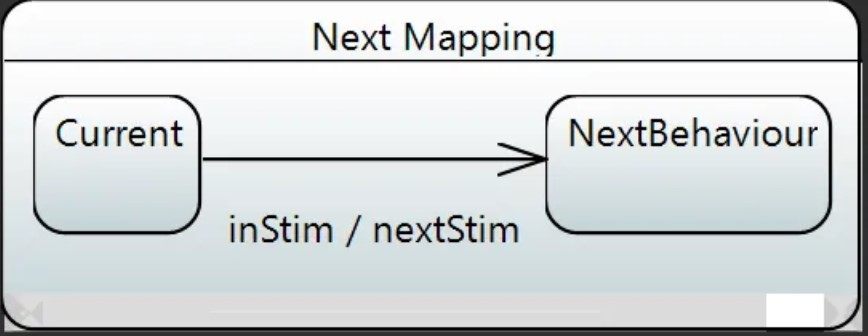
\includegraphics[width=0.5\textwidth]{transitions}
    \caption{A representation of next mappings and their relation to transtions}
    \label{fig:transition}
\end{figure}

\textbf{Sequential States} are super states (state compositions) with a specific composition pattern.
There are at least two inner states.
All inner states are linked by \textit{sequential transitions}.
The sequence has no cycles.
There is a clear initial state with no incoming transitions.
There is a clear final state with no outgoing transitions.
We can see an example sequential state in figure~\ref{fig:sequential}.

\begin{figure}[ht]
    \centering
    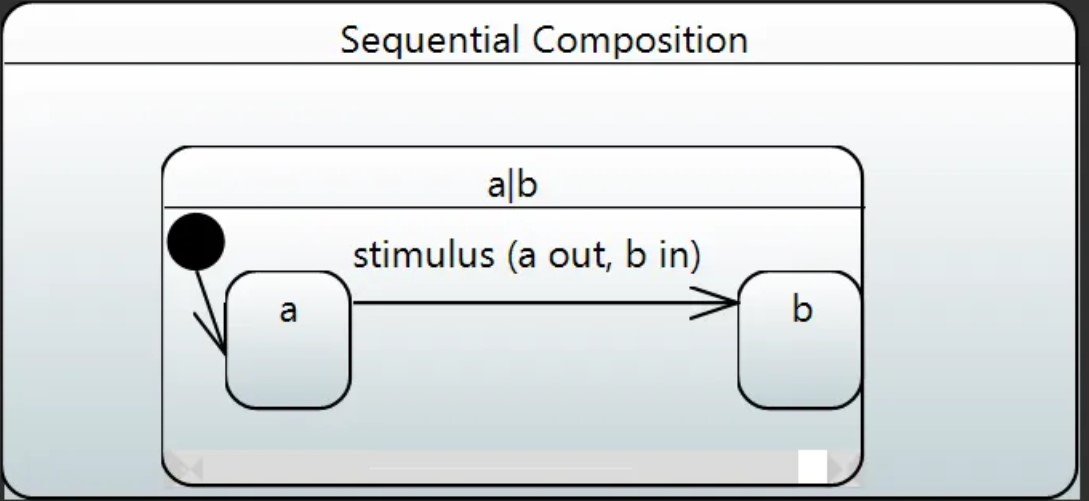
\includegraphics[width=0.5\textwidth]{SequentialBehavior}
    \caption{A C2KA sequential composition represented in a state diagram}
    \label{fig:sequential}
\end{figure}

Note: We explicitly decided not to cover C2KA \textit{parallel compositions} to simplify modelling and parsing.
Instead, a modeller should consider making two different agents which communicate
with each other to model parallel behaviour.

\subsubsection{XMI Parsing}\label{subsubsec:parsing}
Having chosen our input format, we needed to find a way to parse it to be able to process it.
Although XMI is supposed to be a standardized format,
many modelling tools will have slight differences for specific components.
Therefore, creating a parser which can be extended generally to support many tools can be challenging.

Thankfully, this is a general problem others have attempted to solve before, and third-party free libraries exist.
We searched for libraries which supported the most recent UML standards, and we were able to make work.
The libraries we tested were \textit{SDMetrics OpenCore},
\textit{eclipse UML2}, \textit{Apache Xerces}, \textit{XMIParser, by cqframework}, \textit{xmiparser, python}.
We only managed to get the \textbf{SDMetrics} Java library to work within our research period.
Since it adequately met our needs, we did not extend the research period to find other alternatives.

The table below traces user requirements to the parsing choices refining them in this section.
\begin{table}[htbp]
    \centering
    \caption{Parser Requirement Traceability}\label{tab:parse-choice-table}
    \begin{tabularx}{\textwidth}{| l | l | X |}
        % Header
        \hline
        \textbf{ID} & \textbf{User Requirement} & \textbf{Refinement} \\
        % Header end
        \hline
        1 & Input & Use SD Metrics OpenCore library to parse XMI file inputs. \\ \hline
    \end{tabularx}
\end{table}

\newpage
\subsubsection{Target Deployment}
One of our user requirements requires us to target an Operating System.
Just like the choice of modelling tool, we want to avoid the OS target to be a barrier to our tool.
We also want to avoid incurring costs attempting to port our tool across multiple Operating Systems.
\textbf{Java} is a great language which allows us to run the same program on any OS due to the Java Virtual Machine.

We considered \textit{C}, but it is not as simple to make platform independent.
\textit{Python} was also a valid alternative because it is also platform independent.
The deciding factor was the availability of third party libraries.
As mentioned in section~\ref{subsubsec:parsing} The SD Metrics library we use for XMI parsing in our system was implemented in Java.
We were not able to make any alternatives work in Python.
With no particular need for other languages, we decided to keep it simple by only using Java in our program.

The table below traces user requirements to the deployment choices refining them in this section.
\begin{table}[htbp]
    \centering
    \caption{Deployment Requirement Traceability}\label{tab:os-choice-table}
    \begin{tabularx}{\textwidth}{| l | l | X |}
        % Header
        \hline
        \textbf{ID} & \textbf{User Requirement} & \textbf{Refinement} \\
        % Header end
        \hline
        10 & OS Support & Use java for platform independence. \\ \hline
    \end{tabularx}
\end{table}

\newpage
\subsubsection{Architecture Choice}
Choosing how to structure our code depends strongly on our functional requirements,
but quality attributes can play a role as well.
The most relevant quality attributes for the architecture for are scalability and performance.
The other requirements are addressed at different steps of the design process.

To begin with, we can think about what our program does not need, like user interaction during execution.
This already gets rid of the need for user interaction focused patterns like \textit{Model-View-Controller} and its variants.
We also have no need for a server or decentralized processing unless we failed to meet our performance goal on one computer.
We did not expect performance to be an issue big enough to require decentralized processing.
Thus, we can eliminate any server patterns, including \textit{microservice} and \textit{service oriented} architectures.

The initial architecture we chose was the \textit{Layer Pattern}, because it fits quite well with the flow of our program.
We are provided an input, and do a series of unidirectional transformations on it to produce an output at the end.
We believed these transformations made sense as different layers of our program.
Layers could pass their outputs through defined input interfaces of the next layer.
This is great for separation of concerns and maintainability.
It is also a great way to reason about the system allowing us to convert our understanding of C2KA transformation to code easily.

That said, we then realized we were starting to describe a \textbf{Pipe and Filter} architecture.
Instead of layers to transform data, we use filters.
We use pipes as our interface to communicate between them.
We still have great separation of concerns, and the same straightforward reasoning for implementation.
The advantage we gain from this pivot is the ability to increase parallelization of processing compared to the layered architecture.
This allows us to directly improve our \textbf{performance} and \textbf{scalability} by reducing the impact of increased data set sizes.

The table below traces user requirements to the architecture choices refining them in this section.

\begin{table}[htbp]
    \centering
    \caption{Architecture Choice Requirement Traceability}\label{tab:arch-choice-table}
    \begin{tabularx}{\textwidth}{| l | l | X |}
        % Header
        \hline
        \textbf{ID} & \textbf{User Requirement} & \textbf{Refinement} \\
        % Header end
        \hline
        11 & Simple System Analysis Speed & Use parallelization enabled by Pipe and Filter to improve performance. \\ \hline
        12 & Worst Case Mitigation & Use parallelization enabled by Pipe and Filter to reduce scaling costs.  \\ \hline
    \end{tabularx}
\end{table}

\newpage
\subsubsection{Architecture Description}\label{subsubsec:arch-desc}
To describe the concrete implementation of our design,
we will break down the responsibilities of our filters, and the pipes in our system through a visual representation.
In these representations, the filters are the named rounded rectangles.
The directional associations show data flow between filters.
Annotations on the data flows specify what data is contained in the pipe.
We also have forks, which are flows going into a black vertical bar and splitting, showing when data is re-used in parallel.
Joins are the opposite operation, collecting data from independent parallel operations back into one centralized point.
Finally, we have the cloud to indicate a simplification in the diagram.
It explains which details were omitted from the model to make it easier to understand.

Figure~\ref{fig:pipe-1} shows the first part of our architecture model focuses on converting our expected input to a StateDiagram internally.
\begin{figure}[ht]
    \centering
    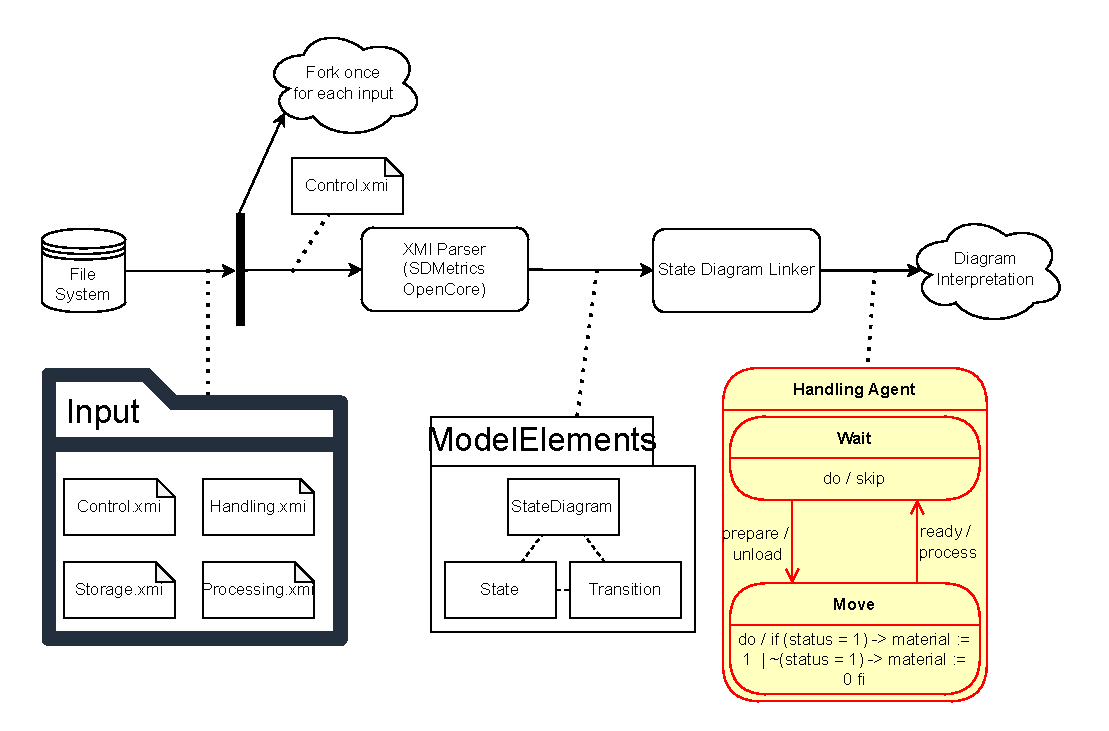
\includegraphics[width=1\textwidth]{pipe-p1.drawio}
    \caption{Converting an XMI file to an internal state diagram representation}
    \label{fig:pipe-1}
\end{figure}

When the program starts execution, it reads all the model files at once from a known input address.
It forks once for each model to process them all in parallel.
The first transformation step is to parse the \textit{XMI file} with our \textbf{XMI Parser}.
The parser uses the SDMetrics library to extract generic UML \textit{ModelElements}.

These elements need to be passed to our \textbf{State Diagram Linker}
to build an internal representation of a \textit{state diagram} for our program.
Specifically, we strongly type model elements according to our internally defined types (states, and transitions).
Super states can be thought of as tree roots, and a state diagram can also be represented as a super state.
This allows us to recursively interpret our diagram just like a tree during the following \textbf{diagram interpretation} stage.

Figure~\ref{fig:pipe-2} shows the  second part of our model completes the process, going from internal StateDiagram to the desired output.
\begin{figure}[ht]
    \centering
    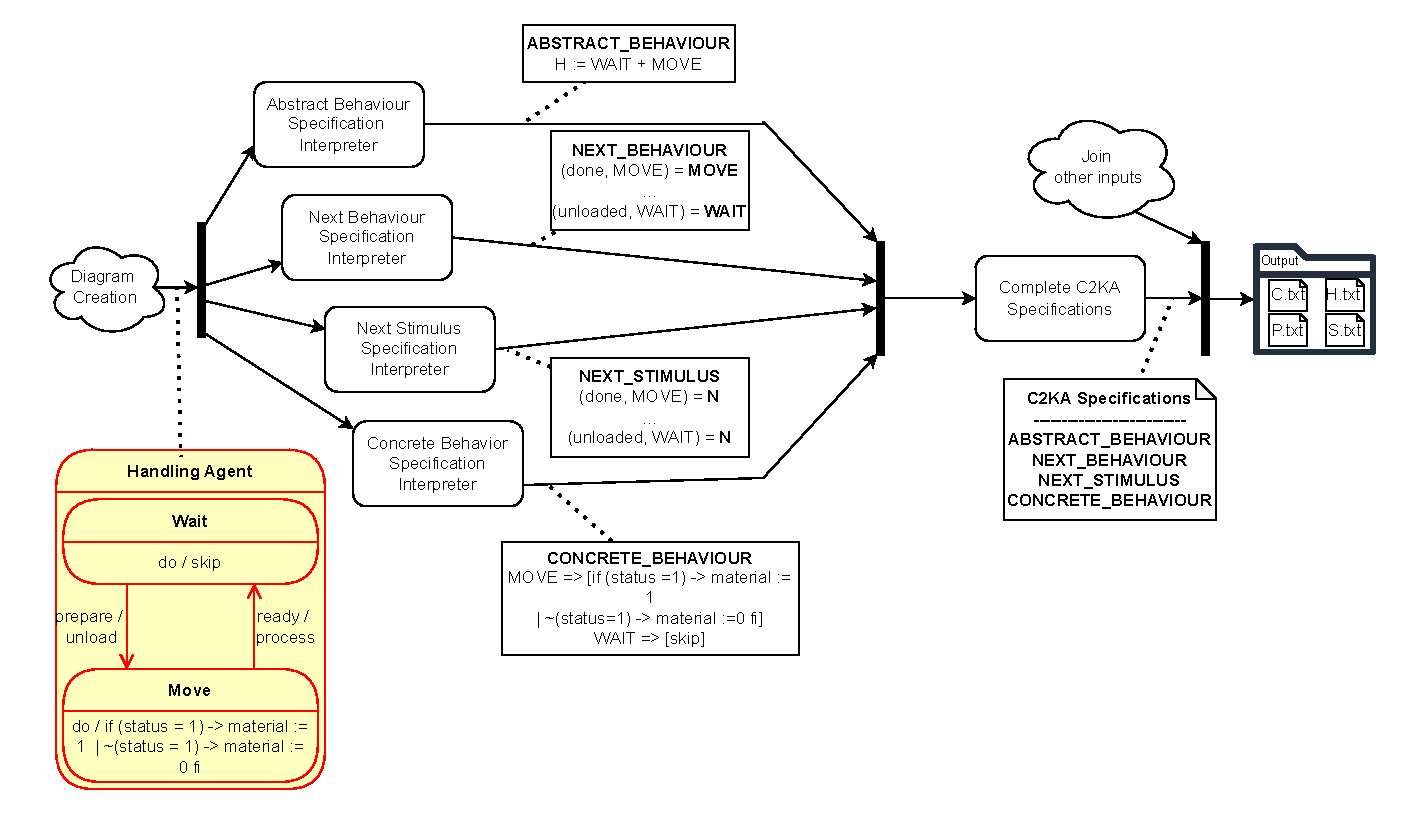
\includegraphics[width=1\textwidth]{pipe-p2.drawio}
    \caption{Interpreting a state diagram to derive a complete C2KA specification}
    \label{fig:pipe-2}
\end{figure}

From our \textit{state diagram}, we can perform different analyses in parallel to find parts of the C2KA specification.
The \textbf{abstract behaviour interpreter} looks at super states to find sequential compositions,
and atomic state names to build a C2KA \textit{abstract behaviour specification}.
States which are not sequentially linked are composed by choice.

The \textbf{concrete behaviour interpreter} simply collects all the atomic behaviours and their doActivities.
The doActivities should already be formatted as the concrete behaviour according to our input specification (section~\ref{subsubsec:input-specification}).
The C2KA \textit{concrete behaviour specification} produced is just a formatted collection of the doActivities of the agent.

The \textbf{next behaviour interpreter} checks transitions to find next behaviour mappings.
A mapping is an initial behaviour, an input stimulus, and the resulting behaviour of the transition.
The \textit{next behaviour specification} is the set of all next behaviour mappings found for that agent.

The \textbf{next stimulus interpreter} is essentially the same as next behaviour,
but instead of the resulting behaviour, we check the output stimulus on the transition.
The \textit{next stimulus specification} is the set of all next stimulus mappings found for that agent.

Once all the interpretation is complete, it gets joined into a complete \textit{C2KA Specification}.
We then need to wait at a barrier for all other models to complete analysis before writing our final \textit{output} to a file.

The reason for the barrier is due to a limitation inherent in C2KA of the next stimulus, and next behaviour functions.
They need to be complete functions,
meaning behaviours in an agent need to have defined neutral mappings for all stimuli in the system.
Neutral mappings being outcomes where nothing changes, a neutral stimulus is sent or the behaviour remains the same.
However, since the view of our system is fragmented across our input set,
we cannot identify all stimuli in the system until we analyze all agent inputs to get a complete view of our system.


The table below traces user requirements to the architecture implementations refining them in this section.
\begin{table}[htbp]
    \centering
    \caption{Architecture Description Requirement Traceability}\label{tab:arch-description-table}
    \begin{tabularx}{\textwidth}{| l | l | X |}
        % Header
        \hline
        \textbf{ID} & \textbf{User Requirement} & \textbf{Refinement} \\
        % Header end
        \hline
        1 & Input & XMI Parser, and State Diagram Linker used to convert input to a diagram format we can interpret. \\ \hline
        2 & C2KA Specifications & Interpreter filters are used to convert a diagram to partial C2KA specifications.
        They are then combined into a full C2KA specification. \\ \hline
        4 & Output & The complete C2KA Specification to output conversion allows us to extract agent text files as output.  \\ \hline
    \end{tabularx}
\end{table}

\newpage
\subsubsection{Project Management}\label{subsubsec:proj-mngmnt}
After user requirements, we described our design choices to cover them.
From design, we needed to create tasks to trace the design to specific code implementation.
To do so, we used \textbf{GitHub Issues} to build a list of upcoming tasks for the project.
In figure~\ref{fig:sampleIssueList}, we show a small sample of these issues completed over the course of the project.
\begin{figure}[ht]
    \centering
    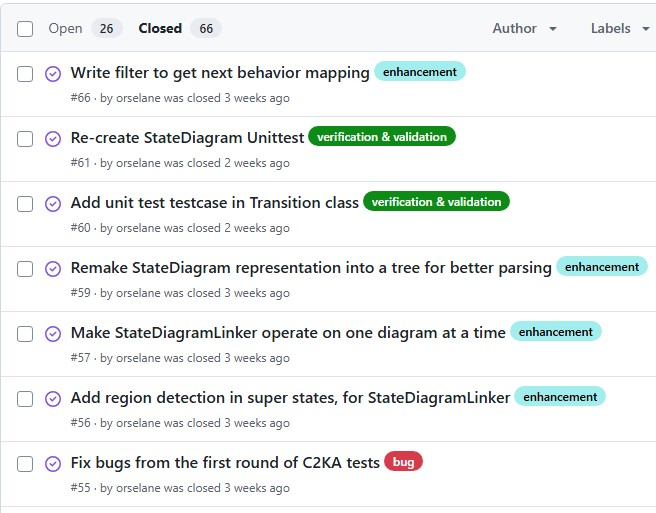
\includegraphics[width=0.8\textwidth]{issueSample}
    \caption{Sample Set of completed issues in our repository}
    \label{fig:sampleIssueList}
\end{figure}

These issues allowed us to assign them when resources were available, and communicate task dependencies easily.
Work done by individuals can be tracked through issues,
preventing multiple people from working on a task simultaneously unaware.
The transition from weekly meetings to asynchronous communication through issues improved our efficiency immensely.
We also customized issue tags to categorize issues
according to our major development concerns, as seen in our repository in figure~\ref{fig:issueTypes}.
\begin{figure}[ht]
    \centering
    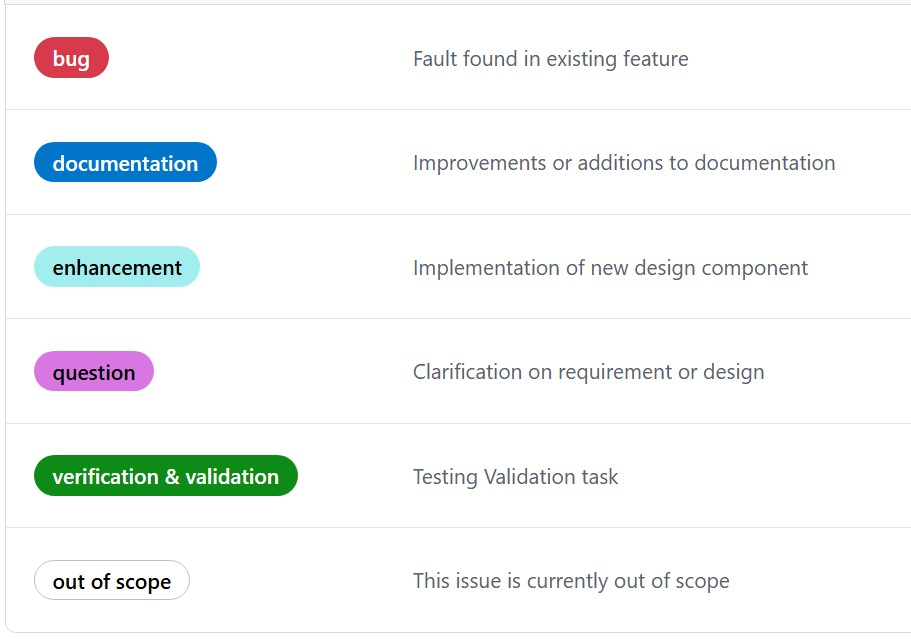
\includegraphics[width=0.8\textwidth]{issueTypes}
    \caption{Types of issues defined in our GitHub repository}
    \label{fig:issueTypes}
\end{figure}

\textit{Enhancements} and \textit{bugs} both relate to implementing our design,
but bugs are errors we found after merging the initial enhancement implementation.
\textit{Verification \& Validation} (V\&V) Tasks related to verifying our code, and validating it.
Usually through creating new tests, but it can also include creating tools for testing,
or establishing and documenting V\&V requirements or strategies.

\textit{Questions} are typically related to clarifications on requirements,
or designs which require research or input from our supervisor.
Once a question is answered, we typically reply directly in the question issue and close it.
Usually, questions have a purpose and can create new issues or unblock existing ones as well.
\textit{Documentation} Tasks related to documenting our project, for any audience.
This includes documentation like this report, function descriptions in code, and a user manual.

\textit{Out of scope} Marks tasks which we identified as out of scope for our current release.
These can include requirements we create to explicitly exclude from the start,
or existing issues we drop later due to time constraints.
In the case where an issue is deemed irrelevant, we do not mark it out of scope.
Instead, we close the issue with a comment for rationale and stop tracking it.
On release, we reset the scope constraints by removing this label on all issues.
After an evaluation of the goals of the next release,
maintainers can decide which issues should stay within the scope of the next release.

We did not develop a great way to automatically trace issues to design,
and we have too many issues to go through them all (over 60 closed issues currently).
Unfortunately, this means we cannot rely on design to code traceability.
Instead, we rely only on testing for validation.
We can, however, demonstrate how we could attempt to manually show traceability through a specific issue.
\begin{figure}[ht]
    \centering
    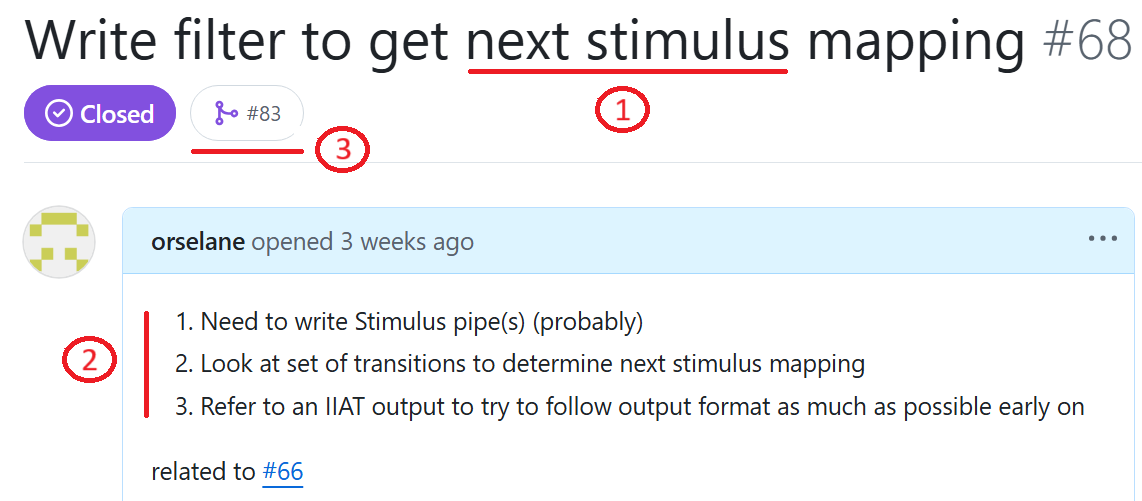
\includegraphics[width=0.9\textwidth]{specificIssue}
    \caption{An annotated enhancement type issue}
    \label{fig:specificIssue}
\end{figure}
In figure~\ref{fig:specificIssue} we can identify from the title (1) the user requirement the issue contributes to.
In this case, it contributes to the C2KA Specification transformations (User Requirement 2).
Then we can look at the description (2) to see a lower level, but informal explanation to guide the code implementation.
Finally, we see the merged branch (3) linking the issue to merged code changes.

\newpage
\subsubsection{Testing Strategy}\label{subsubsec:tests-strat}
Although we never defined a formal test selection criteria,
we defined informal guidelines to define how to verify our code.

For our simplest code unit, \textit{pipes}, we can \textbf{unit test} it.
After construction, we verify public attributes are as expected.

For \textit{filters}, we did \textbf{integration tests} to more closely simulate a real program environment.
For these tests, we called all the filters up to and including the filter under test then evaluated the output.
This allowed us to do iterative development when we developed new filters,
ensuring new filter implementations were not breaking any previously implemented filters.
Figure~\ref{fig:testShowcase} shows how an integration test would like when testing the State Diagram Linker.
\begin{figure}[ht]
    \centering
    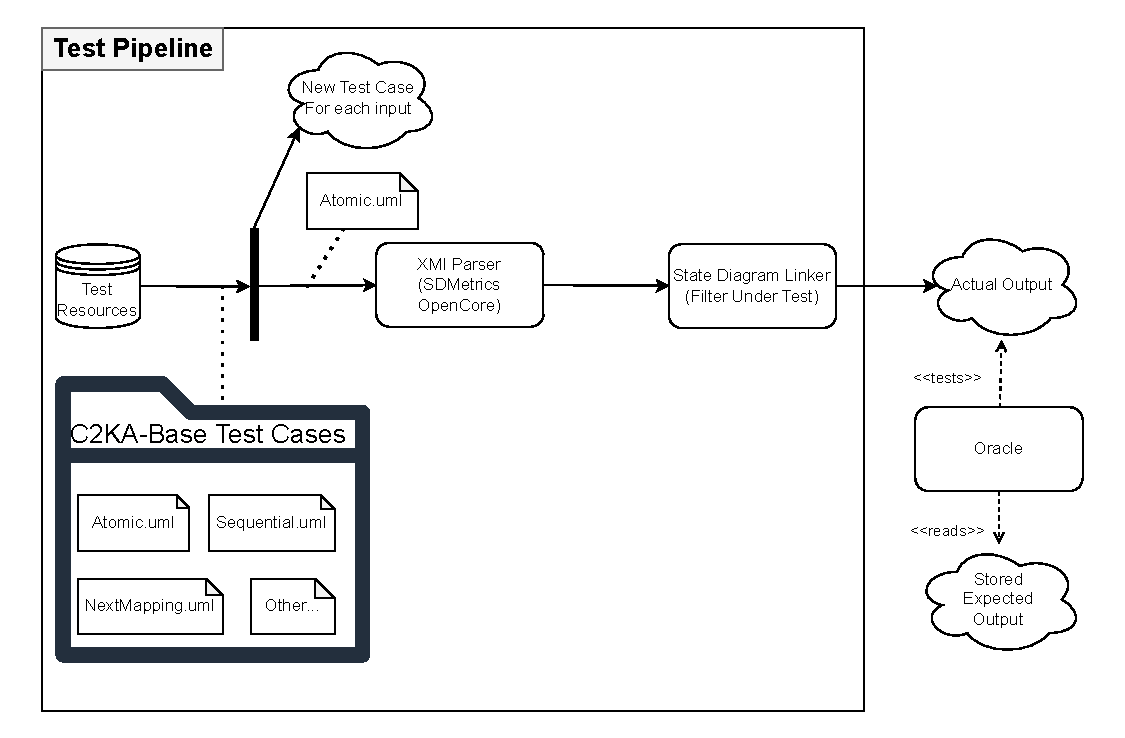
\includegraphics[width=1\textwidth]{testPipeline.drawio}
    \caption{A visualization of the integration test design for State Diagram Linker}
    \label{fig:testShowcase}
\end{figure}

For integration test inputs, we defined a group of elementary C2KA representations which implement
all the elements specified as part of our input specification.
The key diagrams used are the same diagrams included in the input specification section~\ref{subsubsec:input-specification}.

For the complete \textit{C2KASpecification} we did end to end \textbf{system tests}, with a \textbf{custom diff tool}.
To do this, we needed a system with known C2KA outputs.
We got analyzed systems from our supervisor, which we treated as the source of truth.
Then, we also needed to model diagrams representing those specifications.
Finally, we create a test with the diagrams as inputs, the analyzed system as expected outputs,
and compare them with our diff tool.

\begin{figure}
    \centering
    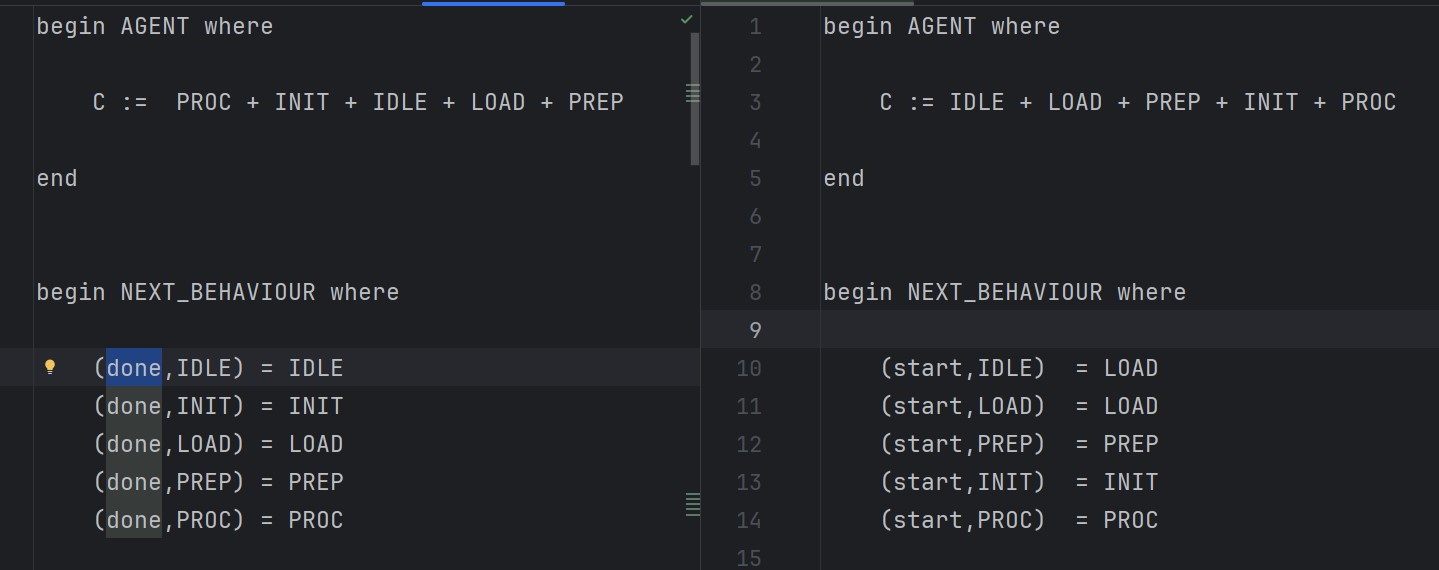
\includegraphics[scale=0.35]{outputDiff}
    \caption{An example of the formatting differences between an actual output (left), and its expected output (right)}
    \label{fig:out-diff}
\end{figure}
In figure~\ref{fig:out-diff}, we see that our produced output files are not exactly the same as the expected output files.
The most glaring difference is the ordering of lines in the NEXT\_BEHAVIOUR spec.
Our tool respects a strict alphabetical order, while the given expected output follows a different formatting rule.
This difference is why we need the diff tool.
Manual C2KA analysis does not follow deterministic formatting rules.
There may be some whitespace differences or a different ordering of lines
which are both semantically irrelevant to the specification.
This is why our diff tool checks for an exact match for lines in a specification type,
regardless of their location within the block or any whitespace.

Figure~\ref{fig:faultinjection} displays what happens when we inject a fault to force a failure.
\begin{figure}
    \centering
    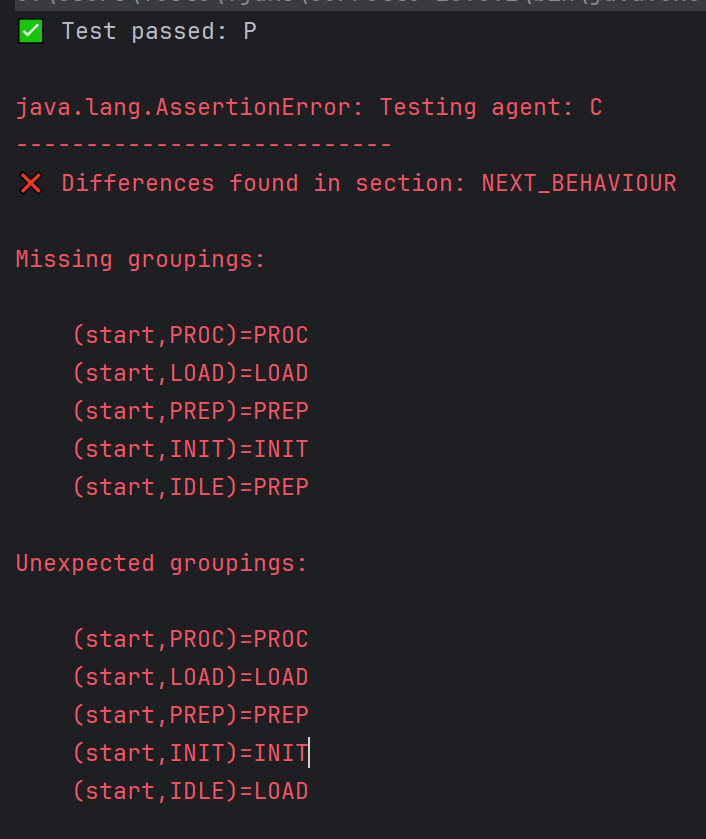
\includegraphics[scale=0.35]{faultinjection}
    \caption{The test result after injecting a fault by modifying a line of the expected output}
    \label{fig:faultinjection}
\end{figure}

We can observe the success case at the top, displaying a checkmark for agent P\@.
When failing, if our actual produced output is missing a line, the diff mentions a grouping is missing.
If we have an additional unexpected line, the diff adds it to the unexpected grouping display.
In the case of a modified line, it will appear in both categories.
A limitation of the current diff tool is it displays errors in groupings instead of displaying specific lines.
Only the (start,IDLE) line was modified in Figure~\ref{fig:faultinjection}, but all start responses got flagged at once.

The table below traces user requirements to our testing strategy concepts refining them in this section.
\begin{table}[htbp]
    \centering
    \caption{Testing Strategy Requirement Traceability}\label{tab:test-strat-table}
    \begin{tabularx}{\textwidth}{| l | l | X |}
        % Header
        \hline
        \textbf{ID} & \textbf{User Requirement} & \textbf{Refinement} \\
        % Header end
        \hline
        15 & Verification Testing & Unit tests, Integration tests provided confidence that our code was continuously functional as we progressed. \\ \hline
        16 & Accurate Outputs & The system tests and diff tool were part of our validation activities to verify output accuracy. \\ \hline
        17 & No False Positives & The system tests should show failures if an output could not be completed, otherwise the diff tool should raise an error. \\ \hline
    \end{tabularx}
\end{table}
\newpage
\subsubsection{Validation Results}\label{subsubsec:test-validation}
For our actual system \textit{functionality}, it only makes sense to test it \textbf{transitively}.
That is, we test it indirectly, in the context of other non-functional requirements.
They serve as the metrics against which to evaluate how well that functionality is fulfilled.
As such, we will analyze our validation strategies for the requirements we managed to fulfill.

We can safely assume our \textit{Portability} is working if we manage to run the application.
Ideally, we should have set up a continuous deployment environment for multiple target operating systems to ensure this property.
For our current scope, we were satisfied with the assumption that
\textbf{Java's JVM} was enough to ensure cross-platform support.

For our \textit{Usability} requirement, we can verify it by looking at the usage instructions.
As we will describe in section~\ref{subsubsec:exec}, the user only needs to \textbf{double-click} the executable to run the program.
To provide the models, they simply drop them in an Input folder, before even executing the program.
We deemed this requirement fully fulfilled from this simple analysis.

For \textit{Compatability} requirements,
we will verify them by generating our \textbf{test inputs} from our supported choices.
As long as our tests work using these inputs, and we have sufficient tests, we prove the compatibility.
It is only to prove support for multiple tools for example that we need to generate more test case inputs from those other tools.
We were not able to add support for multiple options for any of the compatability requirements.

For the \textit{Accuracy} requirement, this is where our \textbf{diff tool} comes into play.
We created accuracy focused \textbf{system tests} as described in section~\ref{subsubsec:tests-strat}.
With a trusted expected output, if we prove an equivalency with the files our tool generates, we can trust it is accurate (at least for that test case).
Unfortunately, we only managed to complete one system test.
Although we marked accuracy as adequately fulfilled, the assurance level is not very high.
Still, at least our accuracy validation is reproducible.
To validate this test case yourself in our repository, run the file located under ``src/test/java/sinks/ManufacturingCellTest''.
In figure~\ref{fig:acc-test}, we can see our diff tool reporting a successful C2KA generation for the Manufacturing Cell system.

\begin{figure}
    \centering
    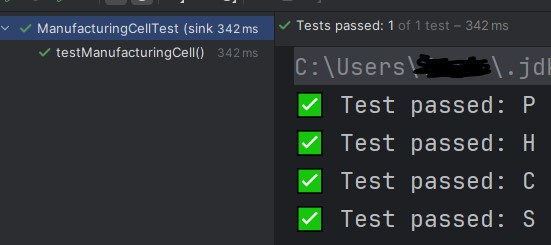
\includegraphics[scale=0.7]{systemTestSuccess}
    \caption{The accuracy system test for the Manufacturing Cell reporting a full success.}
    \label{fig:acc-test}
\end{figure}

We did not manage to write test cases for our diff tool itself, therefore it is valid to doubt the report accuracy.
When debugging, or when we were trying to initially gain confidence in the diff tool, we did manual diffs.
This is a tedious process, and it is very easy to miss things.
To verify the raw diagrams, we can look in the test folder's resources as uml files under ManufacturingCell.
The test folder has the expected outputs as text files, which are the same as the ones from the IIAT repository~\cite{repo_iiat}.
We have a diagrams repository to store the additional files required to load them in papyrus for visual inspection if needed~\cite{repo_diagram}.
If we wished to compare the actual outputs generated in testing, they are generated under the Output folder.
It is unsustainable for new users to do this as well to gain confidence.
Tests for the diff tool itself are important as well.
It is a critical part of the tool chain, and validating it should not be ignored in future work.

The table below traces user requirements to our testing results refining them in this section.
\begin{table}[htbp]
    \centering
    \caption{Validation Requirement Traceability}\label{tab:test-res-table}
    \begin{tabularx}{\textwidth}{| l | l | X |}
        % Header
        \hline
        \textbf{ID} & \textbf{User Requirement} & \textbf{Refinement} \\
        % Header end
        \hline
        1 & Input & Tested transitively as part of other validation activities. \\ \hline
        2 & C2KA Specification & Tested transitively as part of other validation activities.\\ \hline
        4 & Output & Tested transitively as part of other validation activities.\\ \hline
        5 & Minimal User Actions & User simply double-clicks to fully execute the program once configured.\\ \hline
        6 & Modelling Tool Support & Test inputs generated using chosen modelling tool.\\ \hline
        7 & Modelling Language Support  & Test inputs generated using chosen modelling language.\\ \hline
        8 & Diagram Type Support  & Test inputs generated using chosen diagram type.\\ \hline
        10 & OS Support & Rely on the Java JVM for built-in cross-platform support.\\ \hline
        16 & Accurate Outputs & System tests using the diff tool for comparison checks against expected verified outputs. \\ \hline
    \end{tabularx}
\end{table}

\newpage
\subsubsection{Unsatisfied Requirements} \label{subsubsec:unsat-reqs}
As we progressed in the project, some lower priority requirements had to be cut to reduce the scope.

For functional requirements, this meant the \textbf{IIAT Parameters}.
Although these are nice to have, they may have required support for an additional diagram type for small benefits.
The core goal of our program was producing the C2KA Specification transformation.

For non-functional requirements, we completely dropped \textbf{cross tool integration}.
It seemed complex, yet not essential to prove one version of our program was functional.
We also cannot claim \textbf{performance} nor \textbf{scalability} of our program due to lack of testing or proofs.
In theory, these properties should hold with our current design, but we did not take the time to prove it.
We did not complete \textbf{User Documentation} adequately, instead focusing on building a comprehensive report.
The user manual should have been the essential sections of the report a user should be aware of,
formatted in a way which makes it easy to learn about and use our project.
We did not prove that we prevent \textbf{False Positives} either.
False positives are concerned with preventing indeterministic outputs from generating.
This means to satisfy this requirement,
we needed to prove errors get raised in diagrams which lead to indeterministic interpretations.
Our system tests are only focused on accuracy; they assume an output is generated but may be inaccurate.

We also completed some non-functional requirements but in a way that could be improved.
Our parser allows for multiple \textbf{modelling tool support}, but it still needs to be tested.
Similarly, we could have potentially supported multiple \textbf{modelling languages} with little extra effort.
The same may apply to \textbf{diagram types}.
All of this requires additional tests, and may lead to small tweaks increasing our scope beyond what we could handle.

\textbf{Maintainer documentation} is good, but it is not systematic.
There is no automatic way to detect missing documentation to ensure full functional coverage.
It may also have been good to have a maintainer manual alongside the user manual.
It could explain design decisions and the program architecture at a lower level than the report for overarching context.
For now, this report serves adequately for a system specification.

Our custom diff tool was also not systematically tested.
This means the reports we rely on for accuracy validation may be inaccurate themselves due to an unknown fault in the diff tool.
If we had more time, getting better assurance of our diff tool itself would increase our assurance in the program's
\textbf{Accuracy}.

In summary, OS Support, Usability, and the main functions are the only requirements we have fully covered (green).
All other requirements are either adequately covered (also green), or not covered (gray),
as seen in our user requirement table, table~\ref{tab:user-reqs}.


\subsection{Usage}\label{subsec:usage}
\subsubsection{Demonstration Scope}\label{subsubsec:scope}
The demonstration will be using inputs generated to simulate the Manufacturing Cell system seen in section~\ref{subsubsec:c2ka-agents}.
The IIAT tool is pre-configured for this system, and the sample inputs from our V1 release is for this system as well.

To use our tool, we will show the full process from how to generate the inputs up to how to provide them to our target model checker (IIAT) to see the output.
We will assume the reader is familiar with the input specification from section~\ref{subsubsec:input-specification},
and how to create their desired state diagram following the specification.
Therefore, we will start by showing how to export an existing state diagram in Papyrus.

Recall that we already deemed the IIAT-specific properties out of scope in table section~\ref{subsubsec:unsat-reqs}.
For this version of our program, we do not take responsibility for IIAT configurations to run any Model.
We only wish to demonstrate the C2KA specifications are accurate, and can be used irrespective of the modelling tool.
Showing parity with the existing samples for IIAT is the limit of our demonstration.


\subsubsection{Exporting Inputs from Papyrus}
The first step in providing inputs is to export them from Papyrus.
Figure~\ref{fig:export-1}, Figure~\ref{fig:export-2} and Figure~\ref{fig:export-3} will demonstrate the steps required to do so:
\begin{figure}[ht]
    \centering
    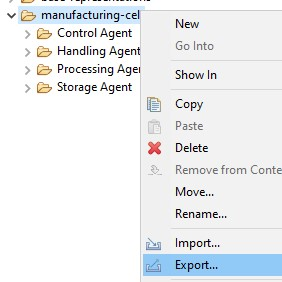
\includegraphics[width=0.5\textwidth]{export-1}
    \caption{Step 1, open export wizard in papyrus}
    \label{fig:export-1}
\end{figure}
\begin{figure}[ht]
    \centering
    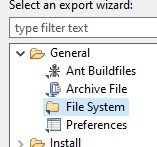
\includegraphics[width=0.5\textwidth]{export-2}
    \caption{Step 2, select file system export}
    \label{fig:export-2}
\end{figure}
\begin{figure}[ht]
    \centering
    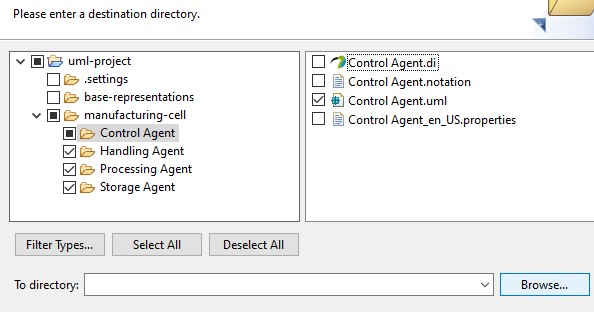
\includegraphics[width=0.5\textwidth]{export-3}
    \caption{Step 3, Select an output directory, and optionally unneeded files.}
    \label{fig:export-3}
\end{figure}

\newpage
\subsubsection{Executing U2C}\label{subsubsec:exec}
To use our program, download the 1.0 zip release from our GitHub~\cite{repo_u2c}.
Then, extract the zip as is to a folder.
Double-click the jar file to execute it (Java 16+ required).
Open the Output folder, there should be four output files corresponding to the sample input.

If the output does not get generated, the program did not succeed.
This is most likely due to an improper Java installation.
Attempt to run the Jar file in the console; for example, on Windows, the command is:
\begin{verbatim}
    java -jar U2C.jar
\end{verbatim}
This should display some error message which is hopefully helpful enough to troubleshoot.
Otherwise, raise a bug on GitHub with steps to reproduce it.
Optionally, contact an individual currently maintaining the tool for help.

If you had no issues, collect the output for use in later steps of this demonstration.
We will use the sample inputs to make the demonstration reproducible.
To analyze your own system, you would remove all files in Input, Output then put your own ``.uml'' files in Input.
Then, execute the program and collect the outputs, just as we did with the sample.

\subsubsection{Running the target Model Checker, IIAT}\label{subsubsec:iiat-run}
To build and run the IIAT, follow the instructions on the IIAT repository~\cite{repo_iiat} to install its dependencies first.
We recommend avoiding windows, it tends to be more difficult to work with.
The next section assumes you have completed the \textit{Installation} section of the IIAT repository's readme file.

Before running the program, it needs to be compiled locally.
When we tried to do so on our Linux installation, the compiler was having trouble loading \textit{hidden} packages.
These were packages that were installed but not explicit dependencies of the project.
To fix this issue, we went into the Makefile and changed the HSFlags variable to add the hidden packages:
\begin{verbatim}HSFlags = -O2 --make -w -package parsec -package vector -package split\end{verbatim}
Admittedly, there must be better fixes, but this was the first time we touched Haskell.
This solution worked well enough to compile and run the program.

Before execution, we also need to configure Maude.
Again, we followed the instructions in the source repository.
The only trouble we had this time was finding the file.
It is not specified, but it is located at /src/MaudeInterface.lhs.

For our particular Arch Linux installation, we also had to add a missing library.
Specifically, we were missing ``libtinfo.so.5''.
We had a ``libtinfo.so.6'' library as a dependency of ncurses (which we already had installed).
It is backward-compatible with the old version, so the solution was to create a symbolic link like so:
\begin{verbatim}sudo link /lib/libtinfo.so.6 /lib/libtinfo.so.5\end{verbatim}

To verify that the program works, run the executable with:
\begin{verbatim}./ImplicitsInteractionsAnalysisTool\end{verbatim}
The pre-configured system should be the manufacturing cell.
If it worked, it should display the intended interactions.
Afterward, the IIAT starts computing the implicit interactions and printing them as it goes.
The tool is very verbose; as such, we only show the output up to the intended interactions in figure~\ref{fig:iiat-out}.
Note that the figure may look strange, but it shows the contents of the real output.
We had to copy the output from our shell because we did not have a way to screenshot it in our host.
\begin{figure}[ht]
    \centering
    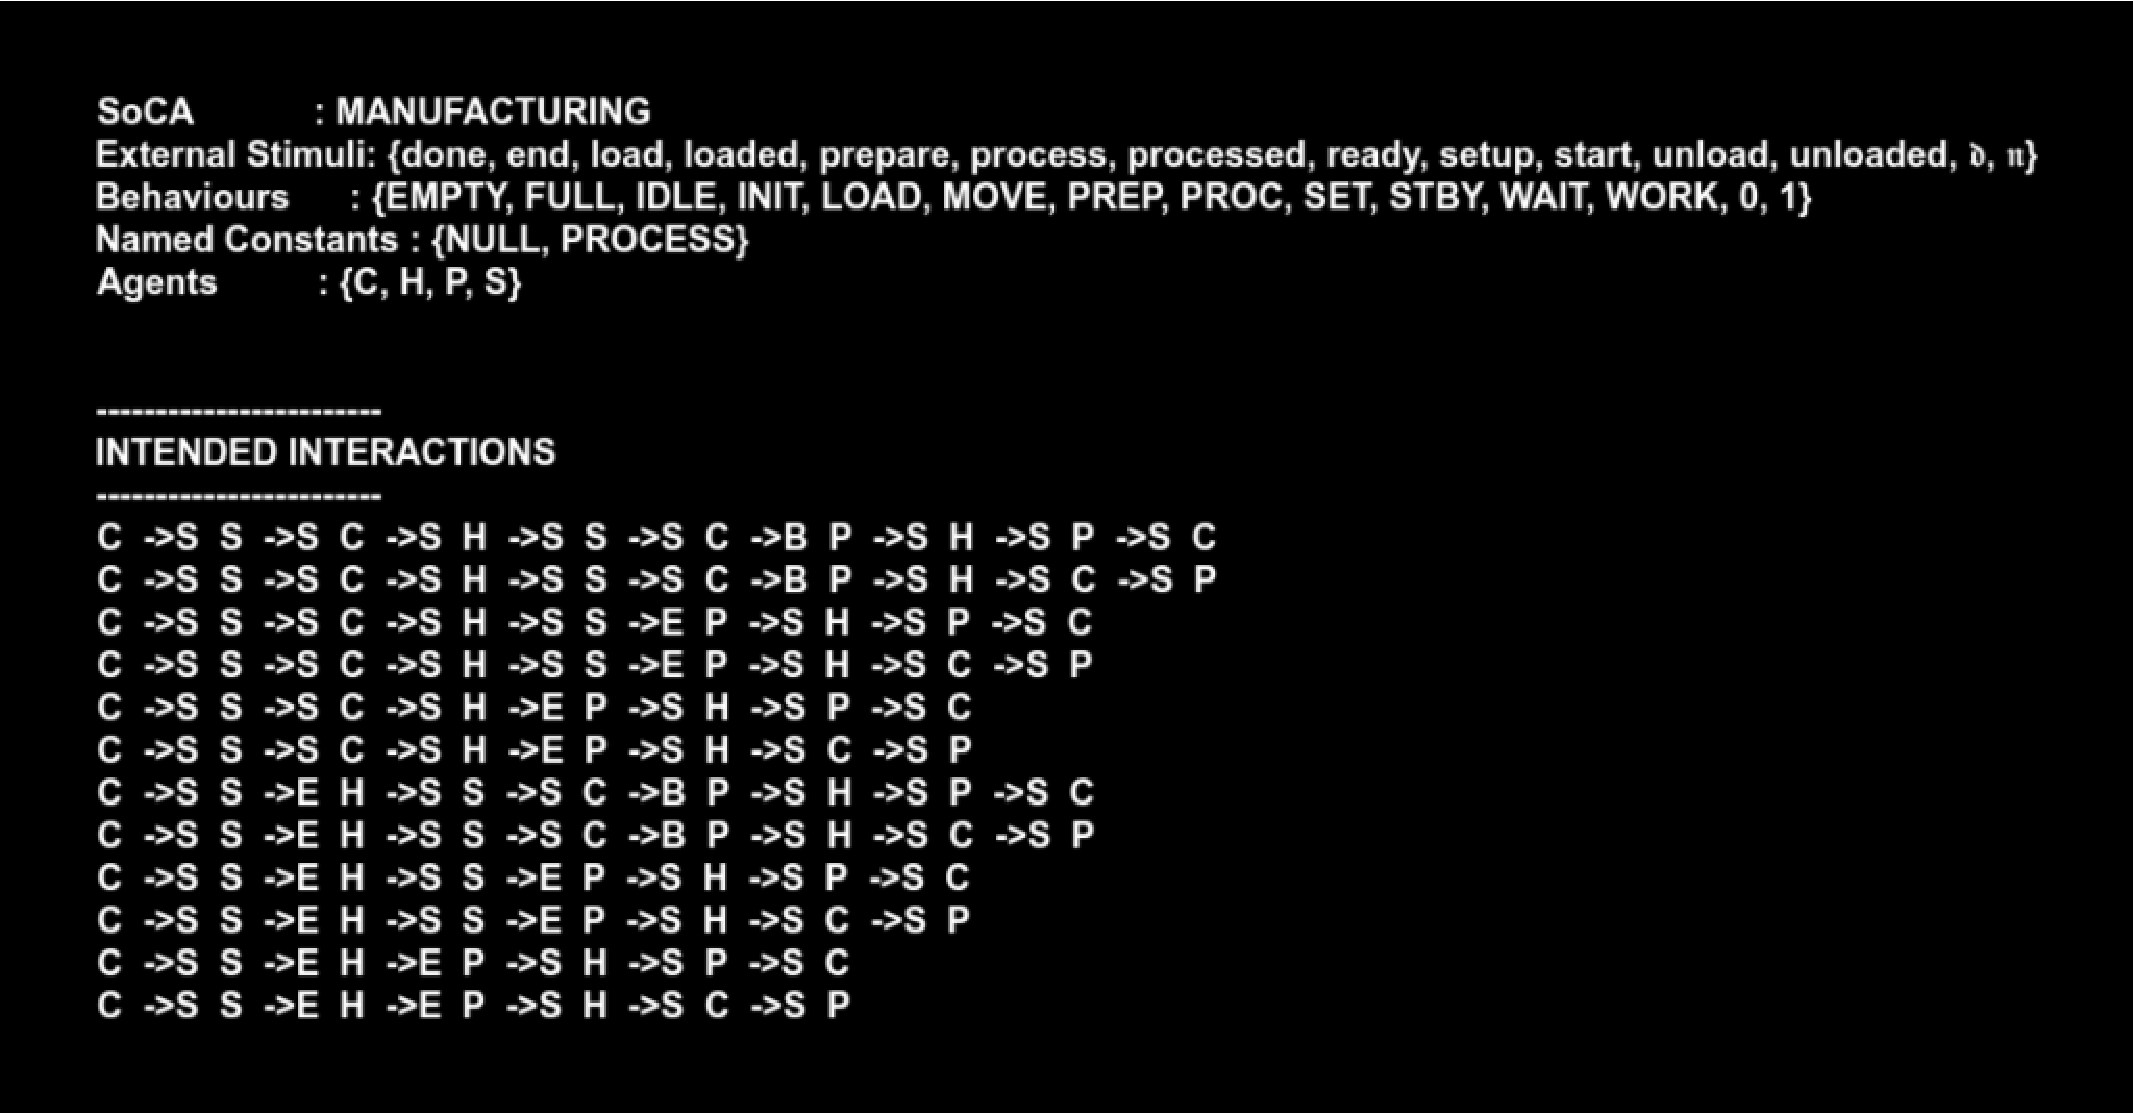
\includegraphics[width=0.6\textwidth]{iiat-out-1}
    \caption{The intended interactions found by the IIAT on the expected input (text copied)}
    \label{fig:iiat-out}
\end{figure}

Note: We did not manage to pipe the output to a file; it currently has to be observed as it prints.
It seems to spawn subprocesses that direct the output to the console directly after the Intended Interactions are printed.
What we did manage to pipe lost its formatting and became difficult to read.
Whichever the case, we believe it to be a limitation of the Linux implementation.
There may be a way through shell commands to redirect the output, but we are not familiar enough with bash.

\subsubsection{Providing generated specifications to IIAT}
Since the IIAT is pre-configured for the Manufacturing Cell,
We can take advantage of that for this demonstration.
Grab the outputs we generated in section~\ref{subsubsec:exec}.
Replace the files under specs/ManufacturingCell with the outputs generated from our sample input diagrams.
The sample input models the Manufacturing Cell, therefore, they should be semantically the same.
You should be able to observe the same outputs from section~\ref{subsubsec:iiat-run} when executing the program again.
Again, due to the verbosity, we only check and display the intended interactions in figure~\ref{fig:iiat-out2}.
The output observed was identical to the expected output in figure~\ref{fig:iiat-out}.
\begin{figure}[ht]
    \centering
    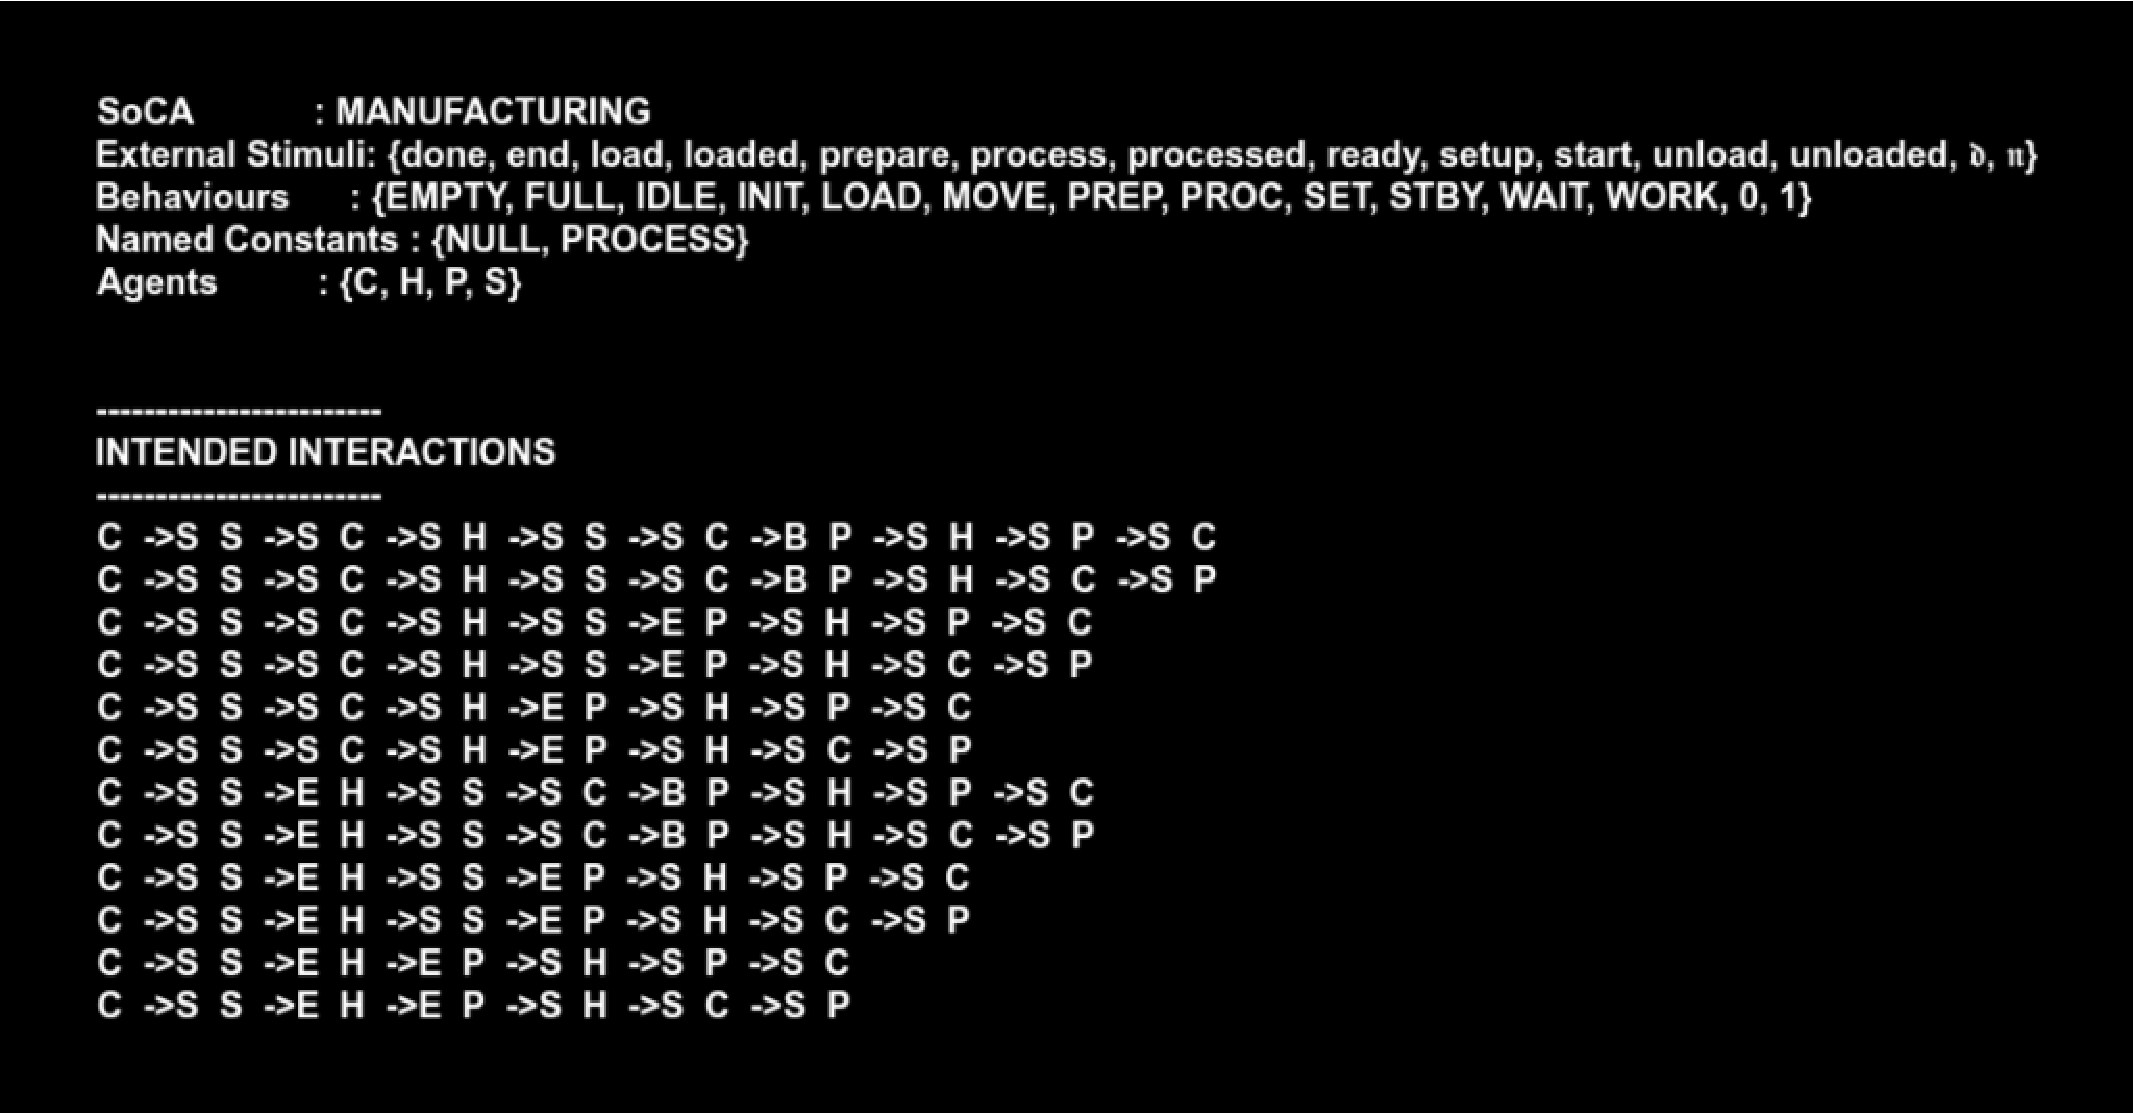
\includegraphics[width=0.6\textwidth]{iiat-out-2}
    \caption{The intended interactions found by the IIAT on our generated specifications (text copied)}
    \label{fig:iiat-out2}
\end{figure}
To analyze different models, additional inputs need to be provided to the IIAT\@.
It does not seem that the IIAT tool explains how to configure the system in the readme.
As such, doing it ourselves for demonstration may require significant exploration.
This is why we deemed it out of scope when we discussed the demonstration scope in section~\ref{subsubsec:scope}.